\chapter{Implementierung}
\label{ch:Implementierung}

In diesem Kapitel wird erläutert, wie die Daten des Datensatzes gesammelt, zur weiteren Verarbeitung vorbereitet und schließlich analysiert werden.
Der Fokus hierbei liegt auf der Implementierung, für mehr Details, siehe Kapitel \todo{link to ref} %verlinke auf kapitel, wo erklärt wird, was wie gemacht wird

\section{App}
\subsection{Plattform}
Die Smartphone-App wurde mit der Sprache Swift für Apple-Smartphones entwickelt. 
Mit der Software XCode lässt sich eine mit Swift geschriebe App kompilieren und auf dem Smartphone installieren.

Zur Einbindung externer Frameworks wird der Dependency-Manager \textit{Accio} und \textit{Carthage} verwendet.
Folgende Frameworks sind in der App eingebunden worden:
\todo{insert table of frameworks with description}

Durch das Framework \textit{Imperio} ist es möglich, die View-Komponenten von der Logik zu trennen. 
Somit ändert sich die Struktur der App, indem jeder Ablauf in der App als \textit{Flow} interpretiert wird. 
Pro Flow wird ein \textit{FlowController} angelegt, welcher die Logik des Ablaufs kontrolliert. 
Ein Flow kann nun beliebig viele \textit{ViewController} starten.
Jede \textit{View}, welche von einem Flow aufgerufen wird, hält ein \textit{Delegate} Objekt.
Ein \textit{Delegate} ist ein Protocol, womit dem \textit{Flow} eine Aktion auf der \textit{View} mitgeteilt werden kann.
Somit wird bei jeder Aktion auf der View eine Funktion des FlowControllers aufgerufen, welcher die View gestartet hat.


Das Framework \textit{Realm} ist eine Datenbank für mobile Systeme, die vollständig auf dem mobilen Endgerät läuft.
Die Daten können direkt als \textit{Objekt} ausgelesen und verarbeitet werden.
In der App wird die Datenbank verwendet, um eine Messung abzuspeichern (siehe Abbildung \ref{implementation:app:erModel}))

Die App ist in 3 Sektionen aufgeteilt, einer \textit{Chartansicht}, einer \textit{Messungsansicht}, sowie einer \textit{Einstellungsansicht}. 
(Abb. \ref{implementation:app:screenshots} Tabbar)
Im weiteren wird nur die \textit{Messungsansicht} genauer erläutert, da die anderen Ansichten im Rahmen der Bachelorarbeit nicht relevant sind.

\begin{figure}[ht]
  \centering
  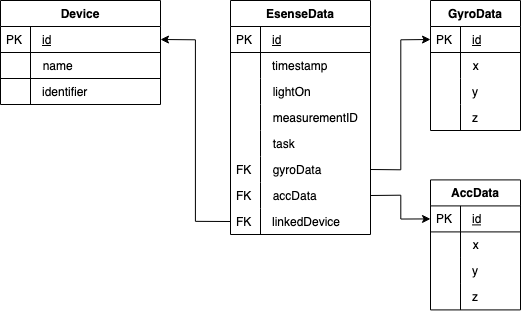
\includegraphics[width=0.7\textwidth]{implementation/app/Database_SleepEar}
  \caption{ER-Diagramm der App-Datenbank\todo{higher resolution}}
  \label{implementation:app:erModel}
\end{figure}

\subsection{Messungsablauf}
Mit der Messungsansicht soll eine komplette Messung durchgeführt werden.
Der \textit{MeasurementFlow} wird gestartet und die erste \textit{View} (Abb. \ref{implementation:app:screenshots:connect_bluetooth}) wird geöffnet.
Nach der erfolgreichen Verbindung mit den eSense-Earpods erfolgt eine Weiterleitung zur nächsten \textit{View} (Abb. \ref{implementation:app:screenshots:user_studies_information}) zum Ausfüllen der Nutzerinformationen. 
Mit dem Betätigen des Buttons: \glqq Start Measurement\grqq bestätigt man die Eingabe der Daten und die Messung beginnt.
Automatisch beginnt der erste Timer (Abb. \ref{implementation:app:screenshots:measurement_started}).
Der Timer zeigt den aktuellen, sowie den nächsten \textit{Task} an, sowie die Restzeit des aktuellen Tasks.
Der genaue Ablauf der einzelnen Timer ist in Kapitel \ref{toRef} \todo{Add ref} detailliert beschrieben.
Nach dem Ablauf des letzten Timers wird eine View geöffnet, welche die Möglichkeit zum Teilen der aktuellen Messung bietet (Abb. \ref{implementation:app:screenshots:sampling_stopped}, \ref{implementation:app:screenshots:share}).
Zudem kann die Datenbank vollständig geleert werden.

\subsection{Messung}
Eine Messung wird im Code in einem \textit{Measurement} Objekt persistiert.
Durch ein Observer-Pattern wird der \textit{MeasurementFlow} über jegliche Änderung informiert und kann entsprechende Handlungen durchführen.
Durch die Funktionen \texttt{startMeasurement} und \texttt{stopMeasurement} kann eine Messung gestartet, bzw gestoppt werden.
Mit der Funktion \texttt{startMeasurement} wird das IMU-Sampling per BLE, sowie die Audioaufnahme gestartet. 
Ebenso wird der erste Timer gestartet und ein doppeltes Lichtsignal gesendet. 
Durch die Funktion \texttt{stopMeasurement} werden die Datenströme gestoppt, ebenfalls ein doppeltes Lichtsignal gesendet und der Timer wird beendet.
Der nächste Task wird gestartet, wenn der Timer abgelaufen ist. Der Timer startet mit der Länge des nächsten Tasks.
Sofern der nächste Task \glqq Hold\_breath\grqq ist, also die Person im folgenden Task die Luft anhält, wird dem Teilnehmer kurz vor Ablauf mitgeteilt, wann der nächste Task startet.
Mit der Instruktion \glqq Bitte die Luft anhalten in 3, 2, 1\grqq \ weiß der Teilnehmer, wann er die Luft anhalten soll.
Durch die Anweisung \glqq Stopp\grqq \ wird dem Nutzer das Ende des Tasks mitgeteilt. 
Die Instruktionen liegen als Audiodatei vor und werden jeweils vor dem jeweiligen Task abgespielt und mittels Bluetooth über die Lautsprecher der eSense-Earpods ausgegeben.

\todo{extend with diagrams like class-diagram}

\section{Anbindung an Auswertungspipeline}
\begin{wrapfigure}{r}{0.2\textwidth}
  \centering
  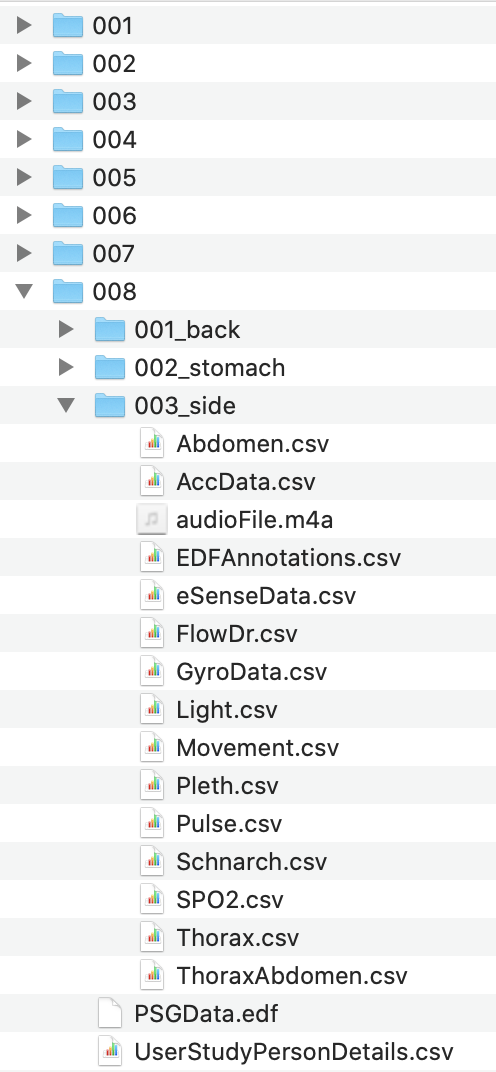
\includegraphics[width=0.15\textwidth]{data_analyzation/folder_structure}
  \caption{Ornderstruktur des Datensatzes}
  \label{implementation:folder_structure}
\end{wrapfigure}
Die App liefert beim Export die Daten der eSense-Earpods, was die IMU-Daten, sowie die Nutzerinformationen und die Mikrofonaufnahme beinhaltet.
Zum aktuellen Stand liegen somit die Daten der eSense-Earpods und vom PSG-System vor. 
Zu Beginn müssen die PSG-Daten, welche als eine Messung für alle 3 Positionen pro Studienteilnehmer persistiert wurde, in 3 einzelne Messungen aufgeteilt werden.
Die Daten des PSG-Systems liegen als \textit{edf}-Datei vor. 
Diese können mittels python und der Library \texttt{edfrd} (siehe \todo{verlinke zu tools}) ausgelesen werden.
Mittels der Funktion \texttt{find\_peaks} aus \texttt{scipy.peak}\ können die Peaks des Lichtsensors ermittelt werden.
Da eine Messung mit 2 Lichtblitzen beginnt und endet, kann nun der Start- und Endzeitpunkt einer Position ermittelt und in die 11 verfügbaren Signale ausgelesen werden.
Pro Position wird nun jedes der Signale als \textit{csv}-Datei im jeweiligen Ordner abgelegt.
Die Daten der eSense-Earpods liegen getrennt in \textit{AccData\_\$ID\$.csv} und \textit{GyroData\_\$ID\$.csv} vor. 
Diese werden ausgelesen und zusammengeführt.
Die Ornderstruktur kann der Abb. \ref{implementation:folder_structure} entnommen werden und ist nun vollständig.

\begin{figure}[ht]
  \centering
  \begin{subfigure}{.25\textwidth}
    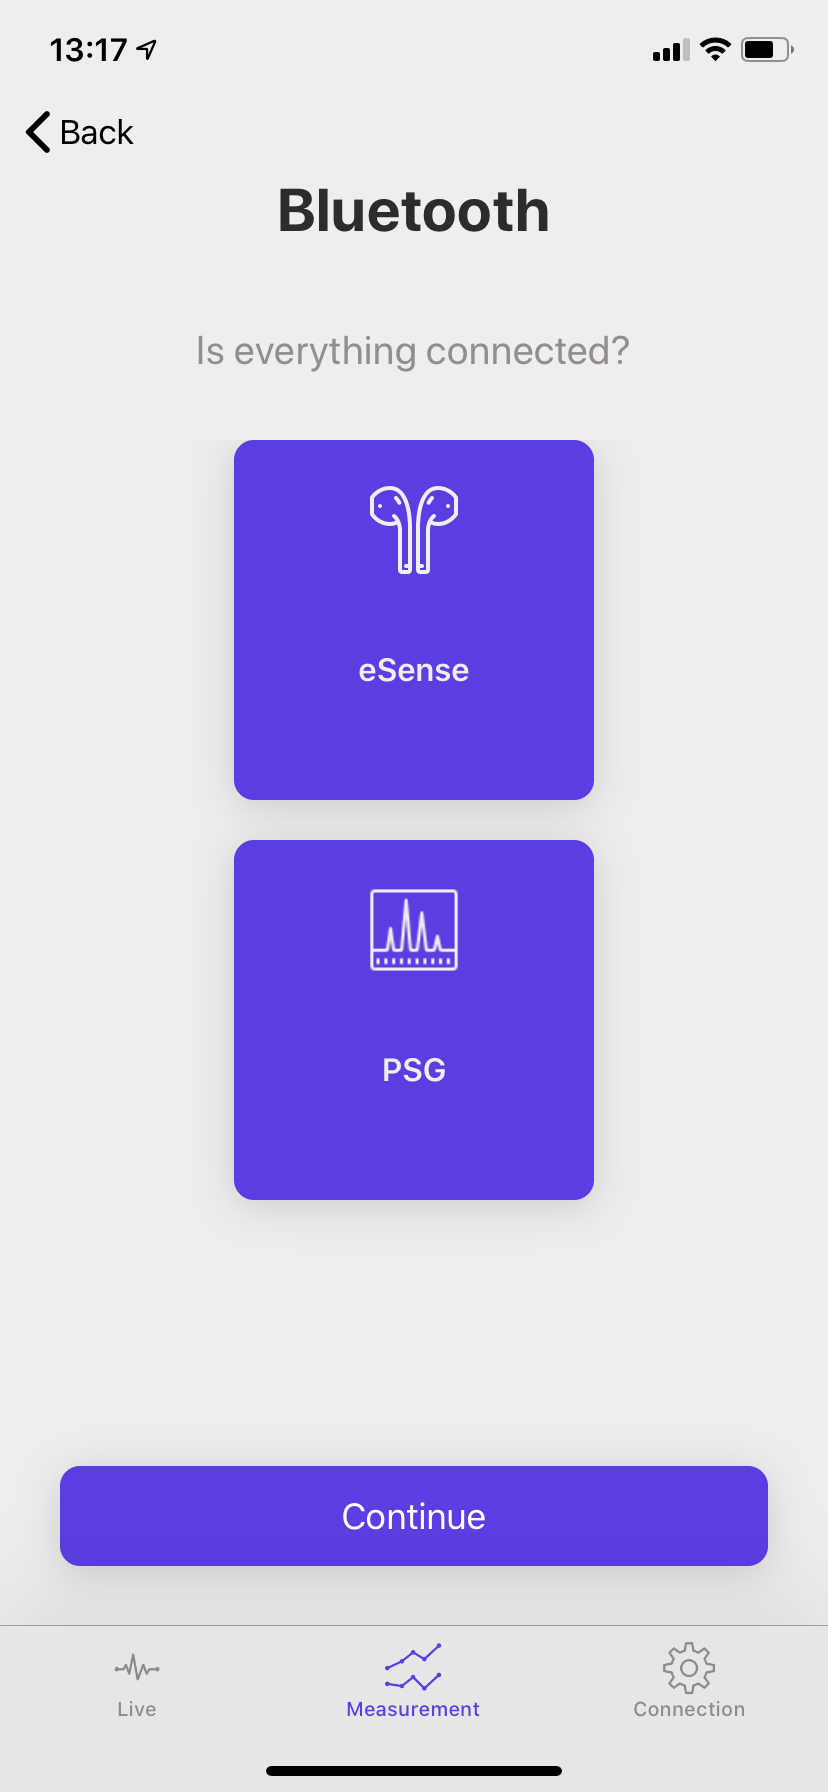
\includegraphics[width=1\textwidth]{app/connect}
    \caption{Verbinden der eSense-Earpods}
    \label{implementation:app:screenshots:connect_bluetooth}
  \end{subfigure}
  \begin{subfigure}{.25\textwidth}
    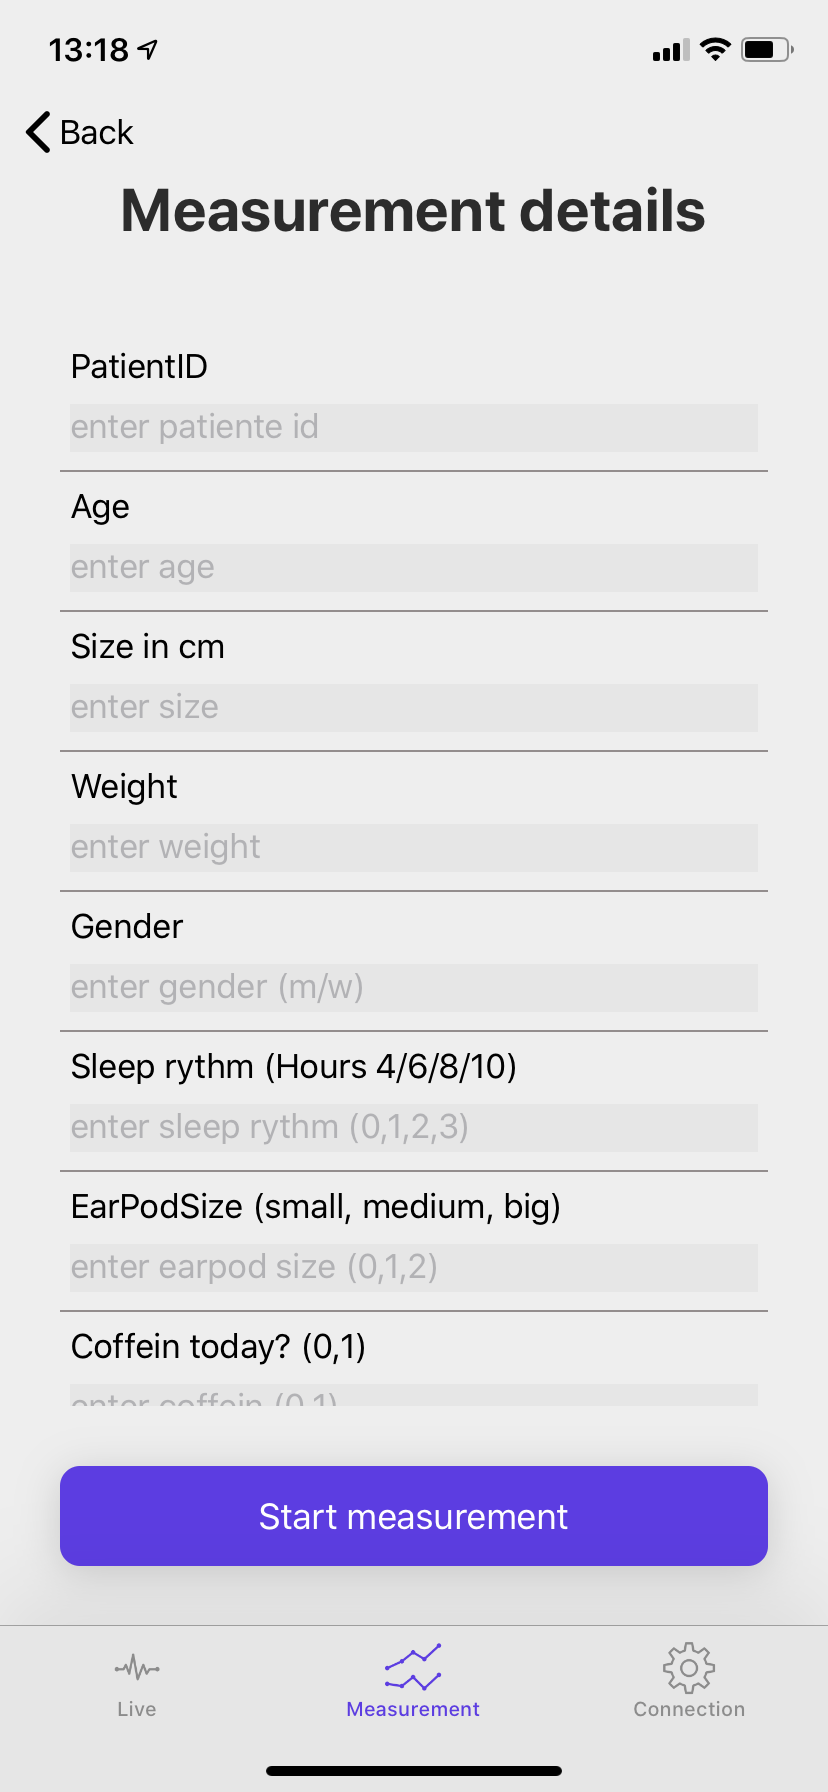
\includegraphics[width=1\textwidth]{app/measurement_details}
    \caption{Eingabe der Nutzerinformationen}
    \label{implementation:app:screenshots:user_studies_information}
  \end{subfigure}
  \begin{subfigure}{.25\textwidth}
    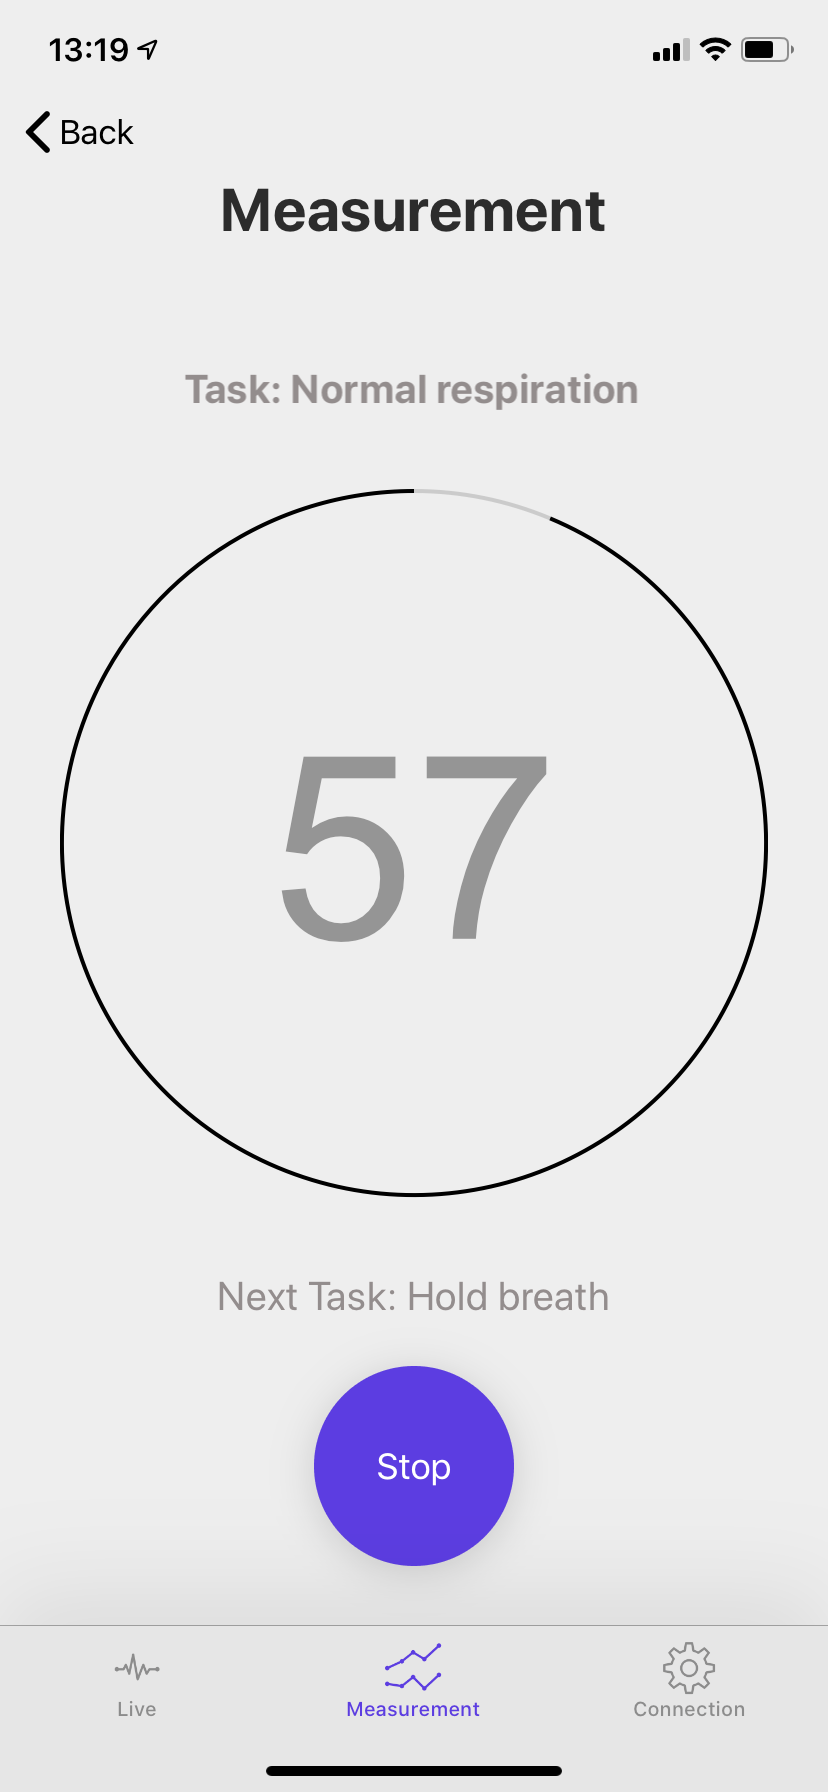
\includegraphics[width=1\textwidth]{app/measurement_timer_02}
    \caption{Messung, aktueller und nächster Task}
    \label{implementation:app:screenshots:measurement_started}
  \end{subfigure}
  \begin{subfigure}{.25\textwidth}
    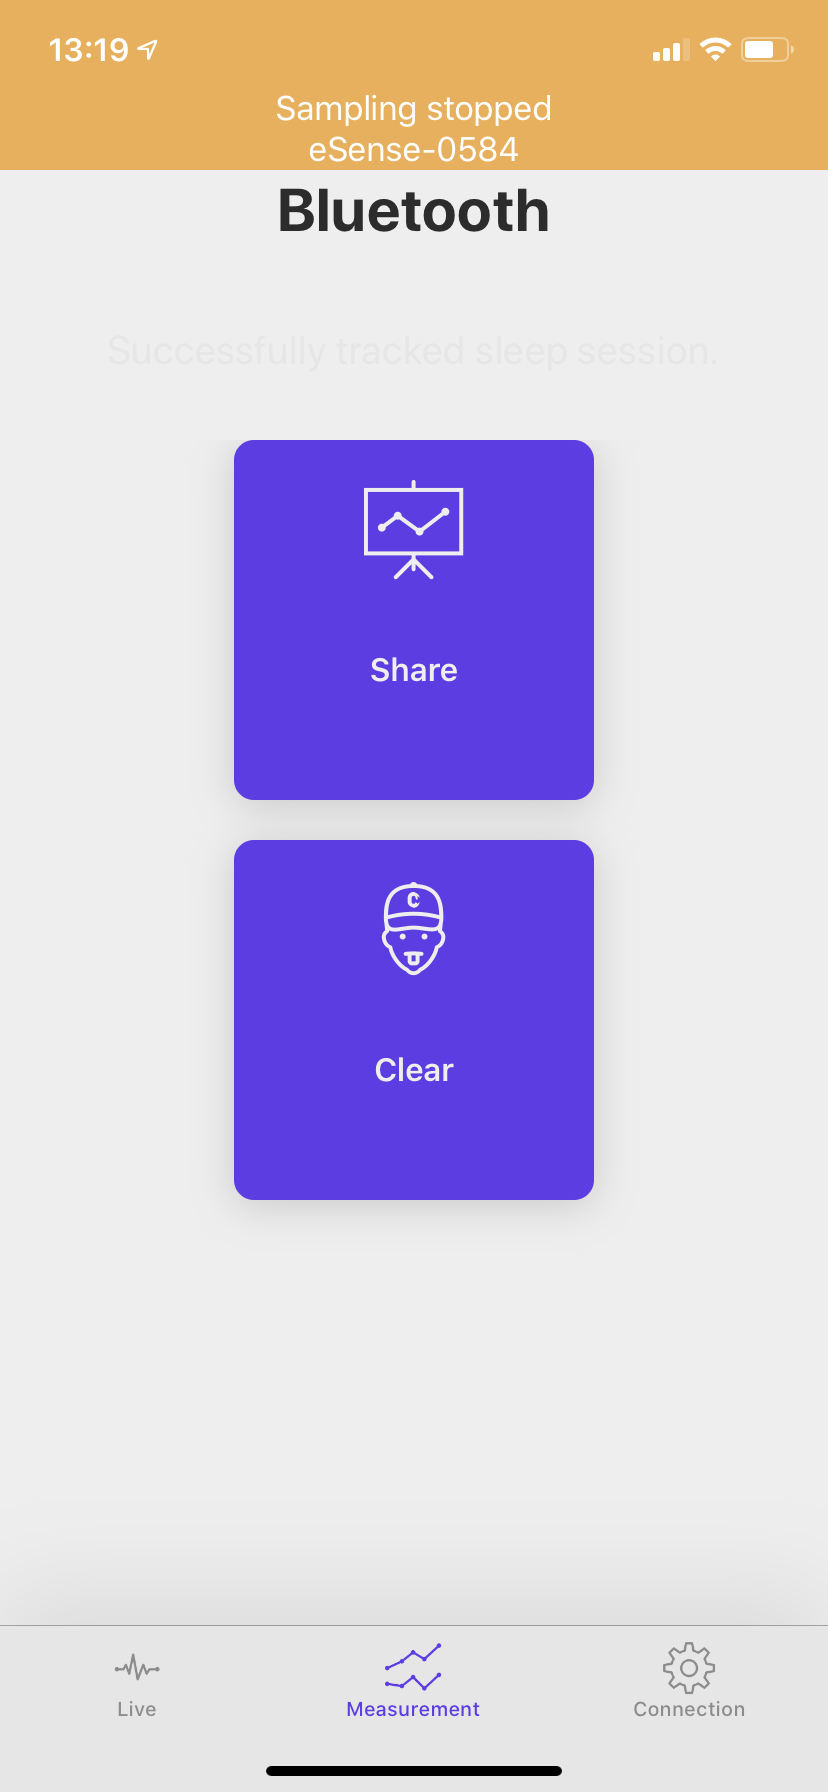
\includegraphics[width=1\textwidth]{app/measurement_finished}
    \caption{Messung beendet}
    \label{implementation:app:screenshots:sampling_stopped}
  \end{subfigure}
  \begin{subfigure}{.25\textwidth}
    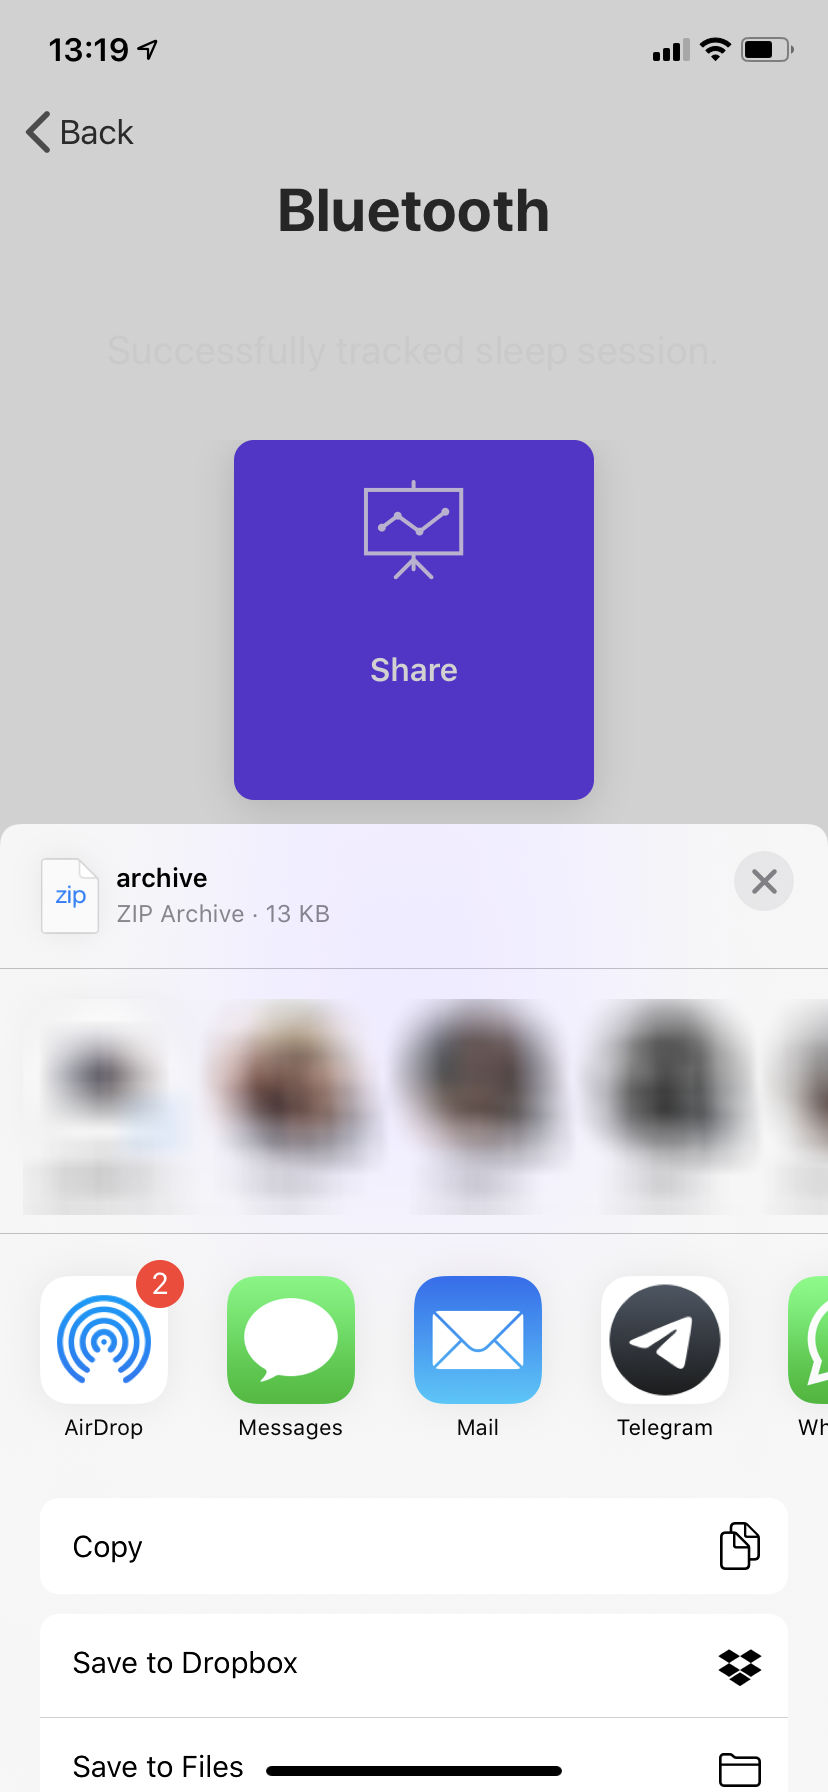
\includegraphics[width=1\textwidth]{app/measurement_share}
    \caption{Messung teilen}
    \label{implementation:app:screenshots:share}
  \end{subfigure}
  \caption{Verlauf einer Messung mit der App}
  \label{implementation:app:screenshots}
\end{figure}

\subsection{Synchronisation der Daten}
Da es nicht garantiert ist, dass der Timer des PSG-Systems zuverlässig arbeitet, wird jeder Peak des Lichtsensors mit dem Lichtsignal der Smartphone-Daten verglichen.
Es wird ein Mittelwert aller Differenzen gebildet und das PSG-Signal wird um diesen verschoben.
Nun ist garantiert, dass die Lichtsignale von PSG-System und dem Smartphone synchron sind. Die Daten sind nun bereit zur Analyse

\section{Verarbeitungspipeline zur Klassifikation}
Wie werden Daten aufgeteilt,wie wird trainiert?
\todo{Fill section}
